\documentclass[letterpaper,twocolumn]{article}

\usepackage[top=1in,bottom=1in,left=0.75in,right=0.75in]{geometry}
\usepackage{graphicx}
\usepackage{newtxtext}
\usepackage{newtxmath}
\usepackage[hyphens]{url}

% Better look for citations that include a section reference like \cite[\S 3]{foobar}.
\usepackage{cite}
\renewcommand{\citemid}{~}

% Load hyperref after other packages.
\usepackage[pdfa,hidelinks,pdfcreator={},pdfproducer={}]{hyperref}
\urlstyle{same}
\def\sectionautorefname{Section}
\def\subsectionautorefname{Section}

% Disable metadata for reproducible PDF.
% https://tex.stackexchange.com/a/313605
\usepackage{ifpdf}
\ifpdf
\pdfinfoomitdate=1
\pdftrailerid{}
\pdfsuppressptexinfo=-1
\fi

% For nice looking check and x marks
\usepackage{pifont}
\newcommand{\cmark}{\ding{51}}%
\newcommand{\xmark}{\ding{55}}%

\hyphenation{Web-RTC}
\hyphenation{Java-Script}

\begin{document}

\date{}

\title{Snowflake, a peer-to-peer censorship circumvention system}

% ANON
\author{}

\maketitle

\begin{abstract}
\begin{itemize}
\item temporary proxies using WebRTC
\item central matching of proxies and clients
\item JavaScript browser add-on, or command-line proxies
\item deployed in Tor Browser
\item history of deployment and blocking attempts
\item observations for circumvention
\end{itemize}
\end{abstract}

% General references:
%   https://gitlab.torproject.org/tpo/anti-censorship/pluggable-transports/snowflake/-/wikis/Technical%20Overview
%   https://www.bamsoftware.com/papers/thesis/#chap:snowflake

\section{Introduction}
\label{sec:intro}

Put Snowflake in context

Spectrum of looks-like-nothing to looks-like-something

Spectrum of few, valuable proxies with careful distribution to
many, cheap proxies with less emphasis on secrecy

\section{Background}
\label{sec:background}

% serene, david

WebRTC

% hooman
- interacting suite of multiple protocols
- example applications
- importantly: built into browsers

flash proxy~\cite{Fifield2012a} (\url{https://bugs.torproject.org/legacy/trac/5578})
% flashproxy.pdf §5.2: "New technologies like WebRTC [24] may fill this need in the future, if they become sufficiently popular that flash proxies' use of them does not stand out as unusual."
uProxy (\url{https://serene.cx/snowflake/})

Comparison with MassBrowser~\cite{Nasr2020a}
% https://github.com/net4people/bbs/issues/32

unfortunate tendency to emphasize the negative aspects of other systems
paints an unnecessarily dire picture
not what we are trying for here
circumvention works, existing systems are successful,
it is a common part of many people's everyday access to the Internet
with Snowflake, we are exploring a different point in the design space

\section{How it works}

\begin{figure*}
\framebox[\textwidth]{\vbox to 2in{\vfil\centering TODO\vfil}}
\caption{
Architecture of Snowflake.
}
\label{fig:architecture}
\end{figure*}

A~Snowflake proxy connection proceeds in three phases.
First, there is the rendezvous, where a client
signals its need for circumvention service
and is matched with a temporary proxy.
Then, there is connection establishment,
where the client and its temporary proxy connect to one another
with WebRTC, using information exchanged during rendezvous.
Finally, there is data transfer,
where the proxy ferries data back and forth
between the client and a remote service
(i.e., a Tor bridge).
\autoref{fig:architecture}
illustrates the process.

The client's circumvention session
does not begin and end with any particular temporary proxy.
Rather, the client strings together
a series of proxies, switching to a new one
whenever an old one goes offline.
This proxy handoff is hidden from the upper-layer protocols
(i.e., the web browser) that use the circumvention tunnel:
to them the Snowflake session appears as one long unbroken connection.

There is an ambient population of temporary Snowflake proxies.
For the most part, these proxies are the web browsers of people who have
installed the Snowflake proxy WebExtension,
or a functionally equivalent headless command-line version.
The proxies periodically poll a centralized server, the broker,
to inquire whether there are any clients that need service.
The broker is responsible for matching and
keeping track of associations between clients and proxies.

A~client begins a Snowflake session by
sending a rendezvous message to the broker.
The rendezvous message must be sent over a blocking-resistant channel,
which may however be slow or expensive; see \autoref{sec:rendezvous} for some examples.
When a client rendezvous message arrives,
the broker chooses one of the immediately available proxies,
subject to NAT compatibility and other matching criteria, % TODO: are there other matching criteria?
forwards the client's rendezvous message to that proxy,
and conveys the client's downstream answer to the rendezvous back to the client.
The client and proxy then initiate a WebRTC connection
with each other; the broker is no longer involved.
Further details on rendezvous will be presented in \autoref{sec:rendezvous}.

The temporary proxy connects both to its assigned client
and to a centralized bridge,
and begins to copy bytes between the client and the bridge
in both directions.
Details about how the connections are established are in \autoref{sec:ice}.
This continues until the client ends its session by disconnecting,
or the proxy goes offline
(which happens, for example, when the web browser where a proxy is running is closed).
When a proxy goes offline,
it does not spell the end of the client's session:
the client and the bridge share end-to-end session state
that persists beyond the lifetime of any single proxy.
The client sends another rendezvous message to the broker,
is assigned another proxy,
and picks up where it left off.
More information about the data transfer phase is in \autoref{sec:data-transfer}.

Never does the client communicate with the broker or bridge directly.
Both the broker and the bridge may be blocked,
from the perspective of the client.
The client only communicates with the broker over an indirect rendezvous channel
that is assumed to be difficult and expensive for a censor to block.
The client only communicates with the bridge via a temporary proxy.
No single temporary proxy is critical to the operation of the system.
A~proxy may be blocked---even while it is in active use by a client---and
clients can adapt by using a different proxy.

\subsection{Rendezvous}
\label{sec:rendezvous}

In the first phase of establishing a Snowflake circumvention session,
the client exchanges a small amount of information with a server
outside the censor's zone of control,
in a process called rendezvous.
It is not possible for a Snowflake client
to establish a peer-to-peer WebRTC connection
with a temporary proxy straight away.
(For one thing, neither the client nor the proxy
know a network identifier for each other at the outset.)
The client and proxy bootstrap a connection between them
by way of a separate blocking-resistant channel
(i.e., something other than WebRTC)
and an intermediary known as the broker.

Rendezvous is not unique to Snowflake;
it is a fairly common component of circumvention designs.
Precedents include the
DEFIANCE Rendezvous Protocol~\cite[\S 3]{Lincoln2012a}
the facilitator interaction in flash proxy~\cite[\S 3]{Fifield2012a},
and the registration proxy in Conjure~\cite[\S 4.1]{Frolov2019b}.
A~key property of rendezvous-using systems
is that they do not rely on any preshared secret information.
The client user needs only to acquire the necessary software;
whatever additional information is required to establish a circumvention session
is exchanged dynamically, at runtime.
A~corollary of the no-secret-information property
is that an adversary---the censor---has
no special disadvantage in attacking the system:
they may download the client software
and then act in every way as a normal user.
This is in contrast to other systems in which,
after acquiring the necessary circumvention software,
a~client must also get ahold of some secret,
such as a password or proxy address,
through an out-of-band channel
presumed to be unavailable to the censor---and
blocking resistance hinges on that secret information
remaining unknown to the censor.
In rendezvous-based systems like Snowflake,
if the censor does not block a proxy server,
it is not out of ignorance,
but because the censor is constrained in some other way,
for example by computational limitations
or fear of collateral blocking.

If rendezvous has the advantage of not requiring secrecy,
its disadvantage is that it presents one more thing to worry about.
Not only the main data transfer channel
but also the rendezvous channel must resist blocking:
the system as a whole is only as secure as the weaker of the two.
The saving grace here is that the security and performance requirements
of rendezvous are different, and generally more lenient.
Rendezvous can afford to be relatively more heavyweight,
slow, expensive, or inefficient for the sake of blocking resistance,
because it accounts for only a small fraction of the overall communication
and occurs only intermittently.
The enlarged design space of rendezvous encompasses
forms of data hiding that would be impractical
for bulk data transfer.
Another helpful consideration is that rendezvous protocols
are separable from the rest of the system.
The assumption of using WebRTC is embedded fairly deeply in Snowflake;
but the rendezvous part is modular,
not coupled to WebRTC or even any single other protocol.

Snowflake rendezvous requires a bidirectional exchange:
the client sends one message to the broker, then receives
one message in reply.
(This is a step backward from flash proxy,
which required only one outgoing message for its rendezvous,
but the communication model of WebRTC makes a reply message unavoidable.)
It is therefore a good fit for request--response protocols,
like those based on HTTP.
We currently support two rendezvous methods in Snowflake:

\begin{description}
\item[Domain fronting]
In this method, the client does one HTTPS exchange
with the broker; however routing through an intermediary such as a CDN
and disguising the externally visible domain name
(the TLS Server Name Indication, or SNI) so that the exchange
appears to be destined to a different site.
We defer to Fifield et~al.~\cite{Fifield2015a}
for a complete description of domain fronting.
\item[AMP cache]
% https://gitlab.torproject.org/tpo/anti-censorship/pluggable-transports/snowflake/-/merge_requests/50
AMP is a framework for web pages written in a restricted dialect of HTML.
Part of this framework is a free-to-use
cache server~\cite{amp-cache}.
Because the cache fetches upstream pages on demand,
it works as a specialized sort of HTTP proxy.
By encoding rendezvous messages as AMP-conformant HTML,
we can use the cache as a proxy for rendezvous,
one that is not easily blocked without blocking the cache server as a whole.
This rendezvous method still requires domain fronting,
because the AMP cache protocol would otherwise expose the
upstream server's domain name in the TLS SNI,
but it increases the number of usable intermediary nodes.
\end{description}

The rendezvous portion of Snowflake is, however, modular,
and any system that can be persuaded to indirectly convey a request
of about 1500 bytes, and a response of about the same size,
can work as a plug-in rendezvous method.
% https://bugs.torproject.org/tpo/anti-censorship/pluggable-transports/snowflake/25594
For example, encrypted DNS
% https://bugs.torproject.org/tpo/anti-censorship/pluggable-transports/snowflake/25874
% \cite[\S 3.4]{Fifield2020a}
(DNS over TLS or DNS over HTTPS):
the client encodes its registration message as a series of DNS queries;
the broker acts as an authoritative resolver;
and a third-party recursive resolver acts as an indirect intermediary,
while DNS encryption hides the broker's domain name in queries
from external observers.
% Flash proxy email rendezvous would not work for Snowflake, because unidirectional.
% https://gitweb.torproject.org/flashproxy.git/tree/flashproxy-reg-email
% https://gitweb.torproject.org/flashproxy.git/tree/facilitator/fp-registrar-email

A~Snowflake rendezvous message is a serialized bundle of data.
Its essential element
is the information necessary to establish a WebRTC connection,
namely a Session Description Protocol (SDP) \emph{offer}~\cite[\S 5]{rfc8839}.
The offer contains information needed for a network connection,
such as the client's external IP addresses;
as well as cryptographic information to secure a later key exchange between the peers.
% Specifically, a certificate fingerprint: https://www.rfc-editor.org/rfc/rfc8122.html#section-5
The rendezvous message also contains the client's
self-measured NAT type, which the broker will use to try to match it
with a compatible proxy.
The client serializes all these pieces of data and sends them to the broker.
The broker chooses an available proxy
and forwards the client's offer to it.
The proxy composes an SDP \emph{answer},
containing its own external addresses and cryptographic information,
and sends it back to the broker,
which then forwards it to the client.
Having exchanged an offer and answer,
the client and proxy are now able to establish a direct WebRTC connection,
without the broker in the middle.
There is more on the mechanics of establishing the connection
in \autoref{sec:ice}.

In WebRTC terms, the offer/answer exchange is called
``signaling,'' and the broker here acts as a signaling server.
While signaling is a necessary component
of any WebRTC-based system,
there is no specified way of doing it.
Every application must invent its own signaling system
according to its requirements
(which for us include covertness and blocking resistance).
Because of the lack of uniformity in accomplishing signaling,
the way a WebRTC application does (or does not do) signaling
may be a distinguishing feature; see \autoref{sec:fingerprinting}
for more considerations along these lines.

\begin{figure}
% TODO: provisional graphic
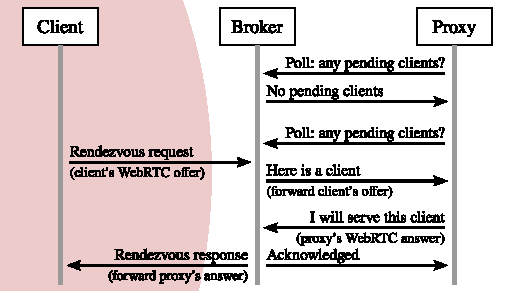
\includegraphics{figures/rendezvous/rendezvous}
\caption{
The long-polling communication model of Snowflake rendezvous.
The assigned proxy connects twice in between the time
the client sends its message and receives the response;
to the client it looks like one roundtrip.
Here, the client's rendezvous method is abstracted;
in reality the censor never contacts the broker directly,
but only via an intermediary.
The shaded background shows the censor's zone of control.
}
\label{fig:rendezvous}
\end{figure}

We use a ``long polling'' model for the client's side of broker interaction.
See \autoref{fig:rendezvous}.
There are proxies polling the broker constantly.
Each poll is an HTTPS request to a designated URL path.
(We assume there is no need for covertness
in the proxies' interaction with the broker,
because this side is outside the censor's observation and control.)
On receiving a poll request,
the broker does not send an HTTPS response immediately,
but waits for a few seconds to see if a client will become available.
If not, the broker sends a response saying ``no clients''
and the proxy sleeps for a while before trying again.
If a client rendezvous does arrive,
the broker extracts the SDP offer and forwards it to the proxy
in the HTTPS response.
The proxy computes its SDP answer,
then sends it back to the broker in a new HTTPS request
(with an attached identifier to permit the broker to match it
with the earlier polling request.)
Meanwhile, the client has been waiting for a response
to its rendezvous message.
The broker encapsulates the proxy's SDP answer
and sends it to the client over the rendezvous channel,
while simultaneously sending an acknowledgement to the proxy.

\subsection{Peer-to-peer connection establishment}
\label{sec:ice}

ICE (Interactive Connectivity Establishment)~\cite{rfc8445}
STUN
DTLS
key exchange
DTLS fingerprint~\cite[\S 5]{rfc8842}

% cecylia
Clients and proxies in the Snowflake network each have one of a few possible
network configurations that can be categorized by two factors:

(1) the mapping behaviour of
the peer's NAT(s), or network address translation tables, and

(2) the filtering behaviour of the peer's firewalls.

There is no guarantee that any two arbitrary peers will be able to form
a connection using STUN for connection establishment as some mapping and
filtering setups are incompatible with each other. Table~\ref{tab:nat-matching} shows
which NAT variations are compatible with each other.
The implementation details of how NATs map internal IP and port combinations
to external ports varies significantly, but for our purposes it was sufficient
to condense these variations together with common firewall filtering behaviour
into the following well-known NAT variations:

\begin{description}
    \item[Full cone] where all connections from the same internal IP address
        and port are mapped to the same external IP and port pair. Any remote
        host can send a packet to an internal host by sending a packet to the
        mapped external IP and port pair.
    \item[Restricted cone] which acts the same as a full cone NAT
        except incoming connections are filtered if there was not a previous outgoing connection
        to the remote IP address.
    \item[Port restricted cone] which acts the same as a restricted
        cone NAT except that incoming connections are filtered if there was not a previous
        outgoing connection to the remote IP and port pair.
    \item[Symmetric] where connections from an
        internal IP and port pair are mapped to an external IP and port pair depending 
        on the remote address. Incoming connections are allowed only if there was an outgoing
        connection to the remote address.
\end{description}


\begin{table*}
    \centering
    \begin{tabular}{l|ccccc}
         & No NAT & Full cone & Restricted cone & Port Restricted cone & Symmetric\\
         \hline
        No NAT & \cmark & \cmark & \cmark & \cmark & \cmark \\
        Full cone & \cmark & \cmark &  \cmark & \cmark & \cmark \\
        Restricted cone & \cmark & \cmark & \cmark & \cmark & \cmark\\
        Port restricted cone & \cmark & \cmark & \cmark & \cmark & \xmark \\
        Symmetric & \cmark & \cmark & \cmark & \xmark & \xmark \\
    \end{tabular}
    \caption{Compatibility of NAT peers for connection establishment with STUN. 
    Pairwise compatible NATs are marked with a checkmark (\cmark) 
    and incompatible NATs are marked with a cross (\xmark).}
    \label{tab:nat-matching}
\end{table*}

As the difficulty lies in compatibility with symmetric NATs, we further simplify
the matching by sorting proxies into one of two pools at the broker: those that work with
symmetric NATs, and those that do not.

We determine the NAT type of snowflake peers differently for clients and proxies, due to the
limitations of browsers and potential censorship vectors that impact client connections.
For clients, we use functionality built into the STUN protocol~\cite{rfc5780}. Not all deployed STUN
servers support NAT discovery; we used a simple script to filter our list of public STUN servers
to include only those that do. We worked with the maintainers of
the pion stun library\footnote{https://github.com/pion/stun} to implement the client side logic
for NAT behaviour discovery, and use this to sort clients into one of two groups.
If the NAT discovery protocol fails, a client will self-report their NAT
type as ``unknown'' to the broker, and the broker assumes these clients to have a symmetric NAT.
Most clients work well with the majority of Snowflake proxies, as
shown in Figure~\ref{fig:clients-by-nat}. However, approximately one quarter of client polls self
report having a symmetric NAT.

\begin{figure}
\centering
    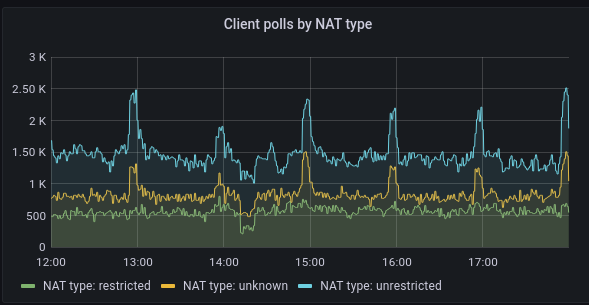
\includegraphics[width=\columnwidth]{figures/clients-by-nat}
    \caption{Snowflake client poll counts by NAT type (placeholder image)}
    \label{fig:clients-by-nat}
\end{figure}

We use a different technique for determining the NAT type of Snowflake proxies because
NAT behaviour is not exposed as part of the WebRTC standard API for web browsers.
Instead, we use a technique similar to that employed by Mass Browser~\cite{Nasr2020a}
and have proxies attempt to establish a connection with a peer behind a symmetric NAT under our
control before polling for clients. If the connection is successful, the proxy will be sorted into
a pool where it will be matched to clients with symmetric NATs. If the connection times out,
the proxy will only be matched to clients without symmetric NATs. Both clients and proxies
retest their NAT type periodically to account for changes in their local networking
environment.

We have a number of
mechanisms in place to avoid too much reliance on single points of failure. If a
proxy is unable to determine its NAT type, we label it as ``unknown'' and assign it only to clients without symmetric NATs. If a proxy
was able to previously determine its NAT type and then fails, it will not transition from a known
NAT type to an ``unknown'' designation. A proxy that has been categorized as suitable for clients
with symmetric NATs, but then fails to connect to too many clients in a row will update its NAT type
and only assigned to clients without symmetric NATs until its next successful NAT check.

The majority of browser based Snowflake proxies do not work with clients that have symmetric NATs.
Due to the have either port restricted or symmetric NATs and are thus not suitable
for restricted clients. Figure~\ref{fig:proxies-by-nats} shows the distribution of proxies by
their NAT pool. Despite this fact, we have managed to maintain a sufficient number of proxies that do
work with symmetric NATs, largely thanks to the option to deploy Snowflake proxies on web servers with
the command line tool.

\begin{figure}
\framebox[\columnwidth]{\vbox to 2in{\vfil\centering TODO\vfil}}
\caption{
Metrics of proxy counts by NAT pool.
}
\label{fig:proxies-by-nats}
\end{figure}


Our ability to perform NAT matching is due to our large proxy pool and the fact that, unlike more
typical uses of WebRTC, we are not trying to form connections between a client and a specific proxy,
but rather to any available proxy that works. Other applications of WebRTC such as video conferencing
platforms, solve the NAT compatibility issue by using TURN or some other way of routing connections
through a centralized point. These approaches are not immediately suitable for Snowflake because
they introduce a central point that can be easily discovered and blocked. We have managed to
provide sufficient capacity for clients with restricted NATs at the moment, but if this capacity
ceases to grow with the increase in users, we could explore the use of TURN servers with rotating
IP addresses to recover from blocking attempts.


WebSocket on the proxy--bridge link
Choice is somewhat arbitrary
Needs to be something supported by browsers
WebSocket easier to use than WebRTC

\subsection{Data transfer}
\label{sec:data-transfer}

% cecylia

Proxies are simple conduits, transferring a reliable stream between endpoints
End-to-end security between client and bridge, proxies untrusted

% hooman
Centralized bridge
- (notionally centralized, though may be realized as multiple instances for performance reasons, see \autoref{sec:experience})

data channels
DTLS
\cite[\S 1]{rfc8831}

% david
Turbo Tunnel~\cite{Fifield2020a}
KCP/smux
- session layer independent of the circumvention channel, permits switching proxies on the fly
- proxy handoff is invisible to upper layers
- the protocol layering generally
browser does not have access to the SCTP layer

Web badge vs. browser add-on vs. standalone daemon
majority browser add-on, more effective at gaining popularity than web badge

\section{Protocol fingerprinting}
\label{sec:fingerprinting}

% kyle, david

\url{https://gitlab.torproject.org/tpo/anti-censorship/pluggable-transports/snowflake/-/wikis/Fingerprinting}

Fifield and Gil Epner~\cite{arxiv.1605.08805}

MacMillan et~al.~\cite{arxiv.2008.03254}

Snowflake leans heavily into the ``address blocking'' side of blocking
resistance, but the ``content blocking'' part is still important.

Fingerprintable features
- signaling
- STUN (choice of servers and contents of messages)
- DTLS
- WebRTC media channel vs. data channel

Historically overvalued in research (cf. \cite{Tschantz2016a})
Practicality is paramount; censors are hard to predict
But we can anticipate possible reactions

\section{Experience}
\label{sec:experience}

\subsection{Deployment history}

% Excerpts from https://gitlab.torproject.org/tpo/network-health/metrics/timeline:
% |2017-01-24|||snowflake|Tor Browser 7.0a1 released, including Snowflake for GNU/Linux only.|[blog post](https://blog.torproject.org/blog/tor-browser-70a1-released)||
% |2017-08-08|||snowflake|Tor Browser 7.5a4 released, including Snowflake for macOS.|[blog post](https://blog.torproject.org/blog/tor-browser-75a4-released) [issue](https://bugs.torproject.org/tpo/applications/tor-browser/22831)||
% |2018-03-26 20:43:42|||snowflake|Release of Tor Browser 8.0a5. Improves snowflake client performance.|[blog post](https://blog.torproject.org/tor-browser-80a5-released) [ticket](https://bugs.torproject.org/tpo/anti-censorship/pluggable-transports/snowflake/21312)||
% |2019-10-01|||snowflake|Release of Tor Browser 9.0a7, the first release that has Snowflake for Windows.|[blog post](https://blog.torproject.org/new-release-tor-browser-90a7) [ticket](https://bugs.torproject.org/tpo/anti-censorship/pluggable-transports/snowflake/25483)||
% |2020-05-22 19:51:29|||snowflake|Release of Tor Browser 9.5a13, the first release with Turbo Tunnel session persistence features for Snowflake. There is a spike in estimated users on 2020-05-21 and 2020-05-22, which appears to be an artifact.|[blog post](https://blog.torproject.org/new-release-tor-browser-95a13) [ticket](https://bugs.torproject.org/tpo/applications/tor-browser/34043) [users graph](https://metrics.torproject.org/userstats-bridge-transport.html?start=2020-03-01&end=2020-08-01&transport=snowflake)||
% |2020-06-02 18:09:48|||snowflake|Release of Tor Browser 10.0a1, the first release with Snowflake for Android.|[blog post](https://blog.torproject.org/new-release-tor-browser-100a1) [ticket](https://bugs.torproject.org/tpo/applications/tor-browser/30318)||
% |2020-06-25|2020-06-25||snowflake|One- or two-day spike in estimated Snowflake users. It resembles the spike that occurred around the time of the Turbo Tunnel release of Tor Browser 9.5a13 on 2020-05-22.|[users graph](https://metrics.torproject.org/userstats-bridge-transport.html?start=2020-03-01&end=2020-08-01&transport=snowflake)|X|
% |2021-07-06 16:56:37|||snowflake|Release of Tor Browser 10.5, first stable release that includes Snowflake.|[blog post](https://blog.torproject.org/new-release-tor-browser-105)||
% |2021-12-20|||snowflake|Release of Tor Browser 11.0.3, with an altered DTLS fingerprint in Snowflake to counteract blocking in Russia.|[blog post](https://blog.torproject.org/new-release-tor-browser-1103/) [issue](https://bugs.torproject.org/tpo/applications/tor-browser-build/40393) [NTC post](https://ntc.party/t/ooni-reports-of-tor-blocking-in-certain-isps-since-2021-12-01/1477/59)||
% |2021-12-14|||snowflake|Release of Tor Browser 11.5a1, with an altered DTLS fingerprint in Snowflake to counteract blocking in Russia.|[blog post](https://blog.torproject.org/new-release-tor-browser-115a1/) [issue](https://bugs.torproject.org/tpo/applications/tor-browser-build/40393) [NTC post](https://ntc.party/t/ooni-reports-of-tor-blocking-in-certain-isps-since-2021-12-01/1477/59)||
% |2022-01-25 17:41:00|||snowflake|Switched the snowflake bridge to a temporary load-balanced staging server. Debugged connection problems until 2022-01-25 18:47:00.|[issue](https://bugs.torproject.org/tpo/tpa/team/40598#note_2772287) [comment](https://bugs.torproject.org/tpo/anti-censorship/pluggable-transports/snowflake/40095#note_2772325) [post](https://forum.torproject.net/t/tor-relays-how-to-reduce-tor-cpu-load-on-a-single-bridge/1483/16) [comment](https://github.com/net4people/bbs/issues/103#issuecomment-1033067920)||
% |2022-03-16 16:51:35|||snowflake|Moved Snowflake traffic to the interim bridge running instances flakey1–flakey8.|[comment](https://bugs.torproject.org/tpo/tpa/team/40664#note_2787624)||
% |2022-07-14|||bridge|Release of Tor Browser 11.5, with a new feature of automatic censorship circumvention configuration.|[blog post](https://blog.torproject.org/new-release-tor-browser-115/)||

The deployment of Snowflake to end users was gradual,
reflecting its development.
It was tested in the alpha release series of Tor Browser
over a course of four years
before finally becoming part of the stable release.
% https://gitlab.torproject.org/tpo/anti-censorship/pluggable-transports/snowflake/-/issues/19001 "First working bundles with Snowflake, for linux only"
The necessary go-webrtc bindings became available first for GNU/Linux,
and so Snowflake was released for the first time, for GNU/Linux only,
with Tor Browser 7.0a1 on \mbox{2017-01-24}.
% https://gitlab.torproject.org/tpo/anti-censorship/pluggable-transports/snowflake/-/issues/19001 "mac reproducible build"
% [tbb-dev] Please check reproducibility of mac build with Snowflake (e084e83418) https://lists.torproject.org/pipermail/tbb-dev/2017-July/000579.html
The next platform for which we got go-webrtc bindings working
and building reproducibly was macOS,
and Snowflake for macOS was released as part of
Tor Browser 7.5a4 on \mbox{2017-08-08}.

% https://gitlab.torproject.org/tpo/anti-censorship/pluggable-transports/snowflake/-/issues/19001 "windows reproducible build"
% https://gitlab.torproject.org/tpo/anti-censorship/pluggable-transports/snowflake/-/issues/25483 "Windows reproducible build of snowflake"
Preparing reproducible the go-webrtc bindings for Windows
presented enormous difficulties.
The Chromium browser from which go-webrtc was derived
% TODO: Maybe "libwebrtc" is better than "Chromium"?
is a massively complex software project,
with a multi-stage and frequently changing build system.
The reproducible build environment,
with its requirements to
cross-compile from source,
without any pre-built binary or proprietary dependencies,
was never a supported build configuration.
The issue stalled us for a long time.
We finally broke through the impasse
by switching from the Chromium-derived go-webrtc
to Pion WebRTC~\cite{pion-webrtc} in the middle of 2019.
% https://gitlab.torproject.org/tpo/anti-censorship/pluggable-transports/snowflake/-/issues/28942 "Evaluate pion WebRTC"
Pion is an independent implementation of WebRTC protocols, written in Go,
that had not existing at the beginning of the Snowflake project.
Pion presented no major difficulties to building reproducibly,
and with it we were able to release Snowflake for Windows
in Tor Browser 9.0a7 on \mbox{2019-10-01}.

While at this point Snowflake was functional on all major desktop platforms,
it was not yet really usable.
The reason is that there was no session persistence:
a~user's Tor browsing session was tied to the first Snowflake proxy they were assigned by the broker.
If the user was lucky, the proxy might persist for an hour;
if unlucky, only a few minutes;
and then the user would have to restart their browser---there was
no way to start using a different proxy on the fly.
(A~lack of session persistence across temporary proxies
had also been a problem in flash proxy~\cite[\S 5.2]{Fifield2012a}.)
Probably because of this, by early 2020,
the number of simultaneous users of Snowflake
had not risen above~40.
% > library(tidyverse)
% > userstats <- read_csv("figures/users-global/userstats-bridge-transport.csv") %>% filter(transport == "snowflake")
%
% Ignoring two apparently anomalous spikes before 2021.
% One on 2020-05-21 and 2020-05-22 (the day of the Turbo Tunnel release):
% > filter(userstats, "2020-05-19" <= date & date <= "2020-05-24")
% # A tibble: 6 x 4
%   date       transport  users  frac
%   <date>     <chr>      <dbl> <dbl>
% 1 2020-05-19 snowflake   9.16   100
% 2 2020-05-20 snowflake  13.6    100
% 3 2020-05-21 snowflake 134.     100
% 4 2020-05-22 snowflake 388.     100
% 5 2020-05-23 snowflake   7.9    100
% 6 2020-05-24 snowflake  13.9    100
% One on 2020-06-25 and 2020-06-26 (not sure what this one is about):
% > filter(userstats, "2020-06-23" <= date & date <= "2020-06-28")
% # A tibble: 6 x 4
%   date       transport users  frac
%   <date>     <chr>     <dbl> <dbl>
% 1 2020-06-23 snowflake  17.0   100
% 2 2020-06-24 snowflake  20.2   100
% 3 2020-06-25 snowflake  71.7   100
% 4 2020-06-26 snowflake 211.    100
% 5 2020-06-27 snowflake  22.5   100
% 6 2020-06-28 snowflake  33.7   100
%
% > filtered <- filter(userstats, !(date %in% c("2020-05-21", "2020-05-22", "2020-06-25", "2020-06-26")))
% > filtered[which.max(filter(filtered, date < "2020-05-21")$users), ]
% # A tibble: 1 x 4
%   date       transport users  frac
%   <date>     <chr>     <dbl> <dbl>
% 1 2020-04-01 snowflake  34.0   100
The Turbo Tunnel session persistence feature
described in \autoref{sec:data-transfer}
became available to users in Tor Browser 9.5a13
on \mbox{2020-05-22}.
% https://gitlab.torproject.org/tpo/anti-censorship/pluggable-transports/snowflake/-/issues/33745 "Merge a turbotunnel branch"
% https://gitlab.torproject.org/tpo/applications/tor-browser/-/issues/34043 "Update snowflake to persist sessions across proxies"
It was at this point that Snowflake became
comfortable enough to use for daily browsing,
% TODO: add NAT matching to this timeline: that was required for comfort as well
and the number of users began to grow steadily into 2021.
Snowflake for Android became available with
Tor Browser 10.0a1 on \mbox{2020-06-02}.
% https://gitlab.torproject.org/tpo/applications/tor-browser/-/issues/28672 "Android reproducible build of Snowflake"

\begin{figure}
% TODO: update users-global chart
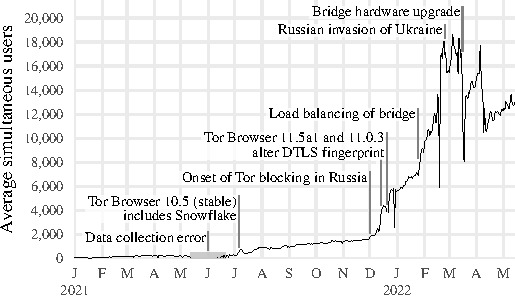
\includegraphics{figures/users-global/users-global}
% TODO: bandwidth chart? ideally with aligned horizontal axis.
\caption{
Estimated average number of simultaneous Snowflake users per day.
The value at the extreme left edge of the graph,
the beginning of 2021, is about~60.
At this point, Snowflake was available in the Tor Browser alpha release series
for desktop platforms and Android,
and it had the Turbo Tunnel session persistence feature.
% Loesing~\cite{tor-tr-2012-10-001} describes how user counts are estimated.
The maximum value in the part of the graph not shown
is 133, on \mbox{2020-12-09}.
% > filtered[which.max(filter(filtered, date < "2021-01-01")$users), ]
% # A tibble: 1 x 4
%   date       transport users  frac
%   <date>     <chr>     <dbl> <dbl>
% 1 2020-12-09 snowflake  133.   100
}
\label{fig:user-counts}
\end{figure}

This brings us to \autoref{fig:user-counts},
which shows the estimated number of Snowflake users since 2021.
Because of Snowflake's affiliation with Tor and Tor Browser,
we estimate users using the normal statistics reported by the bridge
and collected by Tor Metrics.
Be aware: the chart does not show the number of unique daily users,
as one might expect,
but the \emph{average number of simultaneous users} per day.
For example, if the line goes through 1,700 on 2021-12-01,
it means that if the number of Snowflake users were instantaneously sampled
at a random moment in that day, the expected number of users would be 1,700.
The number of unique users per day is necessarily higher,
but how much higher depends on how many hours an average user stays connected.
Counting simultaneous users, rather than unique users,
has been the practice of Tor Metrics since 2012~\cite{tor-tr-2012-10-001};
the reason for it is that the statistics reported by Tor bridges
lend themselves better to the former estimation than the latter.
% TODO: Can we do better with respect to unique users?
% https://bugs.torproject.org/tpo/network-health/metrics/analysis/40012#note_2803514}
The values should not be taken as exact---the
algorithm involves some approximations and guessed parameters---but
the chart is at least relatively comparable to others
produced by Tor Metrics.
% https://bugs.torproject.org/tpo/network-health/metrics/website/40047#note_2796619 "I did some analysis to see what a corrected graph for Snowflake would look like."
% TODO: Speaking of, should we show Snowflake numbers in context with other PTs & relay users?
% https://gitlab.torproject.org/tpo/community/support/-/issues/40050#note_2796770 "This graph shows shows all the Tor users in Russia, whether using relays, bridges, or bridges with pluggable transports."

The growth of Snowflake users began in earnest on
\mbox{2021-07-06}, when it became part of the stable release series
in Tor Browser~10.5.
% https://blog.torproject.org/new-release-tor-browser-105
Being part of the stable series means that it was
available as a built-in option for circumvention for all Tor Browser users,
not only those who had taken the trouble to install a special alpha release.
The rate of adoption increased,
and the number of simultaneous users steadily increased to almost 2,000
over the next five months.

On \mbox{2021-12-01}, some (not all) ISPs in Russia began to block
most forms of access to Tor~\cite{ooni-2021-russia-blocks-tor}.
We will have more to say about this in \autoref{sec:block-ru}.
Snowflake was also affected,
but we released updates to evade the blocking on
\mbox{2021-12-14} (alpha) and
\mbox{2021-12-20} (stable).
The blocking of plain Tor increased demand for circumvention transports,
and Snowflake was strongly affected.
The number of users quadrupled in the next two months.
There were so many new users from Russia, in fact,
that we had to rearchitect the bridge deployment
at the end of January
in order to handle the increased load.
% https://forum.torproject.net/t/tor-relays-how-to-reduce-tor-cpu-load-on-a-single-bridge/1483
% https://bugs.torproject.org/tpo/anti-censorship/pluggable-transports/snowflake/40095#note_2772325
Even with these architectural changes,
the bridge's CPU capacity again became saturated.
Around the beginning of March, Snowflake was almost unusably slow for a few weeks.
% https://old.reddit.com/r/TOR/comments/t49i14/hello_i_have_a_problem_with_snowflake_can_you/
% https://forum.torproject.net/t/tor-project-more-resources-required-for-snowflake-bridge/2353
The invasion of Ukraine by Russia starting on \mbox{2022-03-24}
was accompanied by additional restrictions on Internet access in Russia,
which only increased demand for circumvention.
In response, on \mbox{2022-03-16} we upgraded the bridge to substantial server hardware,
which has been sufficient for the time being.
(See \autoref{sec:future} for an idea to run multiple independent bridge sites,
to permit scaling further.)
As of May 2022, about 65\% of Snowflake users come from Russia.
% https://metrics.torproject.org/collector.html#type-bridge-extra-info
%
% @type bridge-extra-info 1.3
% extra-info flakey3 5481936581E23D2D178105D44DB6915AB06BFB7F
% published 2022-05-20 21:10:47
% transport snowflake
% dirreq-v3-ips ru=12216,us=1640,cn=704,de=400,gb=296,by=272,in=224,??=208,ua=168,fr=160,ir=136,nl=128,ca=88,br=80,it=80,au=72,pl=72,sa=72,es=64,se=64,ch=48,cz=48,mx=48,tr=48,ae=40,jp=40,ro=40,za=40,at=32,eg=32,id=32,co=24,dk=24,dz=24,fi=24,hk=24,hu=24,no=24,ph=24,pk=24,ar=16,bd=16,be=16,cl=16,gr=16,ie=16,il=16,kr=16,kz=16,lt=16,ma=16,mm=16,my=16,ng=16,nz=16,pt=16,sg=16,sk=16,vn=16,al=8,ao=8,az=8,ba=8,bf=8,bg=8,bh=8,bj=8,bo=8,ci=8,cm=8,cr=8,cu=8,cy=8,do=8,ec=8,ee=8,et=8,eu=8,ge=8,gf=8,gh=8,gt=8,hr=8,iq=8,jm=8,jo=8,ke=8,kg=8,km=8,kw=8,lb=8,lk=8,lu=8,lv=8,ly=8,md=8,mk=8,ml=8,mo=8,mu=8,mv=8,mw=8,mz=8,na=8,om=8,pa=8,pe=8,pg=8,pr=8,py=8,qa=8,re=8,rs=8,rw=8,sb=8,sc=8,sd=8,si=8,so=8,sv=8,sy=8,th=8,tm=8,tn=8,tw=8,tz=8,ug=8,uy=8,uz=8,ve=8,ye=8,zm=8
% dirreq-v3-reqs ru=21688,us=2728,cn=1280,de=664,??=648,gb=504,by=464,fr=368,ua=344,in=336,nl=280,ir=248,ca=168,au=152,br=128,it=120,pl=112,es=96,mx=96,ro=96,sa=96,se=88,id=80,ch=72,tr=72,za=72,cz=64,jp=64,ae=56,eg=56,co=48,hk=48,at=40,dk=40,no=40,ar=32,be=32,dz=32,fi=32,ie=32,lv=32,ng=32,nz=32,ph=32,pk=32,pt=32,bd=24,hu=24,il=24,jo=24,kr=24,kz=24,vn=24,az=16,ba=16,cl=16,ec=16,et=16,ge=16,gr=16,hr=16,ke=16,lt=16,ma=16,mm=16,mu=16,my=16,pa=16,sg=16,sk=16,th=16,tm=16,tw=16,uy=16,uz=16,al=8,ao=8,bf=8,bg=8,bh=8,bj=8,bo=8,ci=8,cm=8,cr=8,cu=8,cy=8,do=8,ee=8,eu=8,gf=8,gh=8,gt=8,iq=8,jm=8,kg=8,km=8,kw=8,lb=8,lk=8,lu=8,ly=8,md=8,mk=8,ml=8,mo=8,mv=8,mw=8,mz=8,na=8,om=8,pe=8,pg=8,pr=8,py=8,qa=8,re=8,rs=8,rw=8,sb=8,sc=8,sd=8,si=8,so=8,sv=8,sy=8,tn=8,tz=8,ug=8,ve=8,ye=8,zm=8
% dirreq-v3-resp ok=32240,not-enough-sigs=0,unavailable=0,not-found=0,not-modified=3208,busy=0
% dirreq-v3-direct-dl complete=0,timeout=0,running=0
% dirreq-v3-tunneled-dl complete=27256,timeout=4948,running=32,min=963,d1=112650,d2=280773,q1=417567,d3=637384,d4=13253000,md=22649666,d6=25108500,d7=28307500,q3=31003000,d8=36534666,d9=50908500,max=121278000
% bridge-ips ru=16720,us=2744,cn=1024,de=672,gb=440,by=400,in=400,??=272,fr=264,ua=232,ir=200,nl=200,br=152,ca=152,au=136,it=136,pl=128,sa=112,se=96,tr=96,es=80,jp=80,mx=72,ro=72,ch=64,eg=64,za=64,ae=56,cz=56,at=48,id=48,co=40,dz=40,hk=40,no=40,pk=40,bd=32,be=32,fi=32,kr=32,kz=32,ng=32,pt=32,ar=24,cl=24,dk=24,gr=24,hu=24,ie=24,il=24,ma=24,my=24,ph=24,sk=24,vn=24,bg=16,cu=16,ec=16,gh=16,jo=16,ke=16,kw=16,lk=16,lt=16,lv=16,mm=16,mu=16,nz=16,sg=16,th=16,tw=16,uz=16,ye=16,al=8,ao=8,ap=8,az=8,ba=8,bf=8,bh=8,bj=8,bn=8,bo=8,ci=8,cm=8,cr=8,cy=8,do=8,ee=8,et=8,eu=8,ge=8,gf=8,gn=8,gt=8,hn=8,hr=8,iq=8,is=8,jm=8,kg=8,km=8,lb=8,lu=8,ly=8,md=8,mk=8,ml=8,mo=8,mv=8,mw=8,mz=8,na=8,np=8,om=8,pa=8,pe=8,pg=8,pr=8,ps=8,py=8,qa=8,re=8,rs=8,rw=8,sb=8,sc=8,sd=8,si=8,sn=8,so=8,sr=8,sv=8,sy=8,tm=8,tn=8,tt=8,tz=8,ug=8,uy=8,ve=8,zm=8
% bridge-ip-versions v4=23424,v6=2840
% bridge-ip-transports <OR>=8,snowflake=26264
%
% >>> 21688 / 32240 # dirreq-v3-reqs=ru / dirreq-v3-resp=ok
% 0.6727047146401985
% >>> 16720 / 26264 # bridge-ips=ru / bridge-ip-transports=snowflake
% 0.7137978142076503

% TODO 2022-07-14 Tor Browser 11.5 automatic circumvention configuration https://blog.torproject.org/new-release-tor-browser-115/

% ANON
% The Tor Metrics Timeline~\cite{tor-metrics-timeline}
% has a detailed list of events over the course of Snowflake deployment.

% david
$X$ TB of user data transferred

% cecylia
The deployment of Snowflake proxies began with a bare minimum deployment of three standalone Go proxies all on the same IP address as the Snowflake bridge, as well as a few proxies from deployed Snowflake badges. We began to collect metrics on the number of deployed proxies on \mbox{2019-06-29}. Figure~\ref{fig:total-proxy-counts} shows the total count of unique proxy IP addresses from the beginning of our collection to the writing of this paper. The majority of the growth in Snowflake proxies over the last three years comes from the success of the Snowflake browser add-on. The add-on was released for Firefox on \mbox{2019-06-26} and Chrome on \mbox{2019-07-03}, but the first major spike in proxy counts was thanks to the integration of Snowflake with the existing flash proxy add-on, Cupcake. The number of Cupcake proxies dropped off completely later that year, but Snowflake add-on usage had already risen to compensate. Currently, the vast majority of Snowflake proxies are from the browser add-on, as shown in Figure~\ref{fig:proxy-type-counts}.

While early growth in the number of unique Snowflake proxy IPs was due to the development of easier deployment methods and UX features for proxy volunteers, the later growth in proxy counts were due to outreach and follow the increase in demand for Snowflake proxy capacity from the increase in client usage. 

Counts of web badge vs. browser add-on vs. standalone daemon
Timeline of proxy + webext deployment
% |2019-06-26|||snowflake|Deployed version 0.0.1 of the Snowflake WebExtension for Firefox.|[comment](https://bugs.torproject.org/tpo/anti-censorship/pluggable-transports/snowflake/30931#note_2593598)||
% |2019-07-03|||snowflake|Deployed version 0.0.1 of the Snowflake WebExtension for Chrome.|[comment](https://bugs.torproject.org/tpo/anti-censorship/pluggable-transports/snowflake/30999#note_2593718)||
Cupcake
Relative ineffectiveness of web badge (i.e. the flash proxy model)
people love the add-on and the daily count of connections

Orbot? as both client and proxy?

\subsection{Development challenges}

% arlo, cecylia

Difficulty of using WebRTC outside a browser

Reproducible builds
- difficulty of cross-compiling go-webrtc extracted from Chromium

History of changing domain fronts

scaling
% david
- load balancing
- multi-bridge

The Snowflake system
admittedly contains a lot of moving parts.
Some complexity is inherent in the nature
of what we are building:
Snowflake is more complicated than a static encrypted proxy
and always will be.
Complexity is the enemy of security and robustness, however,
and in a system meant for real production use
could even be considered an existential risk,
if the demands of maintenance exceed what the maintainers can provide.
Managing complexity and designing for low maintenance
are material concerns,
and must sometimes take priority over speed of development.

% Safe Browsing / zip bomb problem (2019)
% https://gitlab.torproject.org/tpo/anti-censorship/pluggable-transports/snowflake/-/issues/31250


\subsection{Blocking in Turkmenistan}
\label{sec:block-tm}

\begin{figure}
\framebox[\linewidth]{\vbox to 2in{\vfil\centering TODO\vfil}}
\caption{
Users in Turkmenistan and Russia,
around blocking events.
}
\label{fig:user-counts-tm-ru}
\end{figure}

% |2021-10-24||tm|snowflake|Snowflake users in Turkmenistan drop to zero, possibly as a result of blocking of the broker's domain-fronting channel.|[issue](https://bugs.torproject.org/tpo/anti-censorship/censorship-analysis/40024) [comment](https://bugs.torproject.org/tpo/community/support/40030#note_2759213) [discussion](http://meetbot.debian.net/tor-meeting/2021/tor-meeting.2021-11-04-15.59.log.html#l-55)|X|

\url{https://bugs.torproject.org/tpo/anti-censorship/censorship-analysis/40024}

\autoref{fig:user-counts-tm-ru}

Block of domain front
Unclear if AMP cache rendezvous was a sufficient workaround
Hard to get testers/volunteers

\subsection{Blocking in Russia}
\label{sec:block-ru}

% https://gitlab.torproject.org/tpo/community/support/-/issues/40050#note_2796770

% mention the creeping block of VPNs? https://github.com/net4people/bbs/issues/76

% david

\autoref{fig:user-counts-tm-ru}

\url{https://bugs.torproject.org/tpo/community/support/40050}
\url{https://ntc.party/t/ooni-reports-of-tor-blocking-in-certain-isps-since-2021-12-01/1477}
% \url{https://blog.torproject.org/tor-censorship-in-russia/}

Snowflake blocked in Russia, along with all other Tor protocols,
in December 2021 \cite{ooni-2021-russia-blocks-tor}
In comparison to TM, easy to get testers
Managed to unblock it within 2 weeks

supported\_groups in Specific DTLS Server Hello Extension
Release to change fingerprint evaded blocking, has worked in Russia since
Had been anticipated by MacMillan et al.\cite[\S 3]{arxiv.2008.03254}
Though not necessarily the wrong call not to have prioritized a fix earlier
Importance during the invasion of Ukraine
- increased usage caused scaling difficulties
  \url{https://forum.torproject.net/t/tor-project-more-resources-required-for-snowflake-bridge/2353}

Second round of DTLS fingerprinting, this time targeting DTLS Client Hello?
\url{https://bugs.torproject.org/tpo/anti-censorship/censorship-analysis/40030#note_2803188}
\url{https://bugs.torproject.org/tpo/anti-censorship/pluggable-transports/snowflake/40140}
\url{https://ntc.party/t/a-new-snowflake-blocking-rule-offset-of-supported-groups-in-dtls-client-hello/2420}

% Iran September 2022
% https://lists.torproject.org/pipermail/anti-censorship-team/2022-September/000247.html

\subsection{SQL injection attempts at broker}

% cecylia

\url{https://bugs.torproject.org/tpo/anti-censorship/pluggable-transports/snowflake/40089}
Actually tailored to the broker protocol, not a generic attack tool.

\subsection{Rate of proxy IP address churn}

% shelikhoo

Need a new experiment for this
\url{https://bugs.torproject.org/tpo/anti-censorship/pluggable-transports/snowflake/34075}

\subsection{Performance}
\label{sec:performance}

% cecylia

\section{Future work}
\label{sec:future}

% shelikhoo

Distributed bridge architecture
\url{https://bugs.torproject.org/tpo/anti-censorship/pluggable-transports/snowflake/40129}

Multiplexing?

% ANON
% \section*{Availability}
%
% \url{https://snowflake.torproject.org/}

% ANON
% \section*{Acknowledgements}
%
% Griffin Boyce
% Chris Ball
% Tor Project
% Sukhbir Singh
% Ivan Markin (AMP cache)
% Pion (who at Pion?)
% ValdikSS (fingerprinting research during Russia blocking)
% Vern Paxson, CDT, OTF, anyone else Serene was involved with?
% Greenhost (eclips.is)
% Arthur Edelstein
% Linus Nordberg
% Mullvad (donated bridge hardware)
% volunteers running snowflake proxies
% anonymous donors

\bibliographystyle{plainurl}
\bibliography{snowflake}

\end{document}
